\documentclass[acmsmall,screen,review]{acmart}

\AtBeginDocument{%
  \providecommand\BibTeX{{%
    Bib\TeX}}}

\setcopyright{acmlicensed}
\copyrightyear{2018}
\acmYear{2018}
\acmDOI{XXXXXXX.XXXXXXX}

\acmJournal{JACM}
\acmVolume{37}
\acmNumber{4}
\acmArticle{111}
\acmMonth{8}

\usepackage{amsmath,amsfonts}
\usepackage{algorithmic}
\usepackage{graphicx}
\usepackage{textcomp}
\usepackage{xcolor}
\usepackage{multirow}
\usepackage{listings}
\usepackage{tcolorbox}
\tcbuselibrary{skins,breakable}
\usepackage{circledtext}
\usepackage{url}
\usepackage{subcaption}

\lstdefinestyle{python}{
    language=Python,
    basicstyle=\ttfamily\footnotesize,
    keywordstyle=\color{blue},
    stringstyle=\color{red},
    commentstyle=\color{gray},
    breaklines=true,
    frame=single,
    numbers=left,
    numberstyle=\tiny\color{gray}
}

\newtcolorbox{insightbox}[1]{%
  enhanced, breakable,
  colback=black!2,
  colframe=black!12,
  boxrule=0.4pt, arc=1pt,
  left=6pt,right=6pt,top=6pt,bottom=6pt,
  before skip=6pt, after skip=6pt,
  title={Insight: #1},
  fonttitle=\bfseries\itshape,
  colbacktitle=black!2, coltitle=black,
  titlerule=0.6pt,
  titlerule style={draw=blue!18},
  borderline west={1.5pt}{0pt}{blue!40}
}

\begin{document}

\title{Pocket Agent: Quantifying On-Device LLM Agent Costs for Edge and Networked Systems}

\begin{abstract}
Recent advances in large language models (LLMs) pave the way for building low-latency, privacy-preserving, and always-available AI assistants.
However, deploying LLM-enabled AI agency on mobile devices remains challenging due to device heterogeneity, limited computational resources, and the complexity of interactions between models and other mobile applications. We present \textbf{Pocket Agent}, a first comprehensive measurement framework that quantifies the real-world costs of LLM agents across edge (mobile and laptop) and cloud (A100) platforms. We instrument a complete agentic loop, where the model selects and invokes tools to gather information or execute code (\textit{Tool}), performs the tool operation (\textit{Action}), and processes the results (\textit{Observation}) iteratively.
Our evaluation of five models (Gemma 3n E2B IT, Llama 3.2 3B, Qwen 3 4B and 0.6B versions, and DeepSeek R1 Qwen Distill 1.5B) reveals a capability threshold. Qwen 3 (4B) benefits from agency strongly, Qwen 3 (0.6B) benefits modestly, while Gemma 3n, Llama 3.2, and DeepSeek R1 do not.
On mobile devices, longer tool-induced prompts cause prohibitive Time-to-First-Token spikes — up to 5 minutes for a 1800-token prompt on an iPhone 15.
We propose energy-per-successful-solution as a practical deployment metric. With this measure, tool-augmented Qwen 3 (4B) raises Pass@1 accuracy from 44.8\% to 79.6\% and Pass@10 accuracy from 58.6\% to 86.9\%, cutting the cumulative energy per solved problem by 53\%.
\end{abstract}

\begin{CCSXML}
<ccs2012>
  <concept>
    <concept_id>10010147.10010178.10010179</concept_id>
    <concept_desc>Computing methodologies~Natural language processing</concept_desc>
    <concept_significance>500</concept_significance>
  </concept>
  <concept>
    <concept_id>10003120.10003138</concept_id>
    <concept_desc>Human-centered computing~Ubiquitous and mobile computing</concept_desc>
    <concept_significance>300</concept_significance>
  </concept>
  <concept>
    <concept_id>10011007.10010940.10011003.10011002</concept_id>
    <concept_desc>Software and its engineering~Software performance</concept_desc>
    <concept_significance>100</concept_significance>
  </concept>
</ccs2012>
\end{CCSXML}

\ccsdesc[500]{Computing methodologies~Natural language processing}
\ccsdesc[300]{Human-centered computing~Ubiquitous and mobile computing}
\ccsdesc[100]{Software and its engineering~Software performance}

\keywords{on-device AI, LLM agents, mobile computing, performance measurement, energy efficiency}

\maketitle

\section{Introduction}
Large language models (LLMs) have demonstrated superior performance across natural language understanding, reasoning, code generation, and multimodal tasks~\cite{10606356,Lu_2025_CVPR}, expanding their adoption in consumer applications like assistants, customer service, education, and healthcare~\cite{10.1145/3580305.3599572,zhao2025surveylargelanguagemodels,thirunavukarasu2023large,milano2023large}.
%As the user base continues to grow,
The deployment of LLMs is transitioning from cloud-based query-response systems to interactive agents that can maintain long-term context, plan multi-step actions, and integrate external tools or services~\cite{li-2025-review}.
This evolution suggests a paradigm shift, i.e., LLMs are shifting from passive knowledge sources to proactive decision-making entities embedded in daily life.

Deploying LLM agents on resource-constrained devices in pervasive environments, such as smartphones, wearables, edge servers, and IoT devices reduces cloud dependency, enabling stronger privacy, reduced latency, offline availability, and personalization through locally collected contextual data. However, on-device execution of LLMs requires rethinking of runtime and deployment design of LLM systems, since the computational and memory demands of LLMs often exceed the capabilities of mobile platforms~\cite{8876870}.

Yet, despite rapid progress in optimizing single-shot inference performance \cite{mlc-llm}, no prior study has, to our knowledge, measured the complete agentic workflow, where models repeatedly invoke tools, process observations, and maintain context on real consumer devices.
Unlike single-shot inference, agentic usage introduces iterative \textbf{Tool→Action→Observation} loops. For example, when solving a coding problem, the model selects a code execution tool (\textit{Tool}), runs a test (\textit{Action}), receives feedback (\textit{Observation}), and iterates with corrections. These loops amplify latency, memory, and energy consumption on resource-constrained devices.
This gap leaves critical system-level questions unanswered: What is the true cost of agentic loops in real-world environments? Under what conditions do tool invocations actually improve task success or efficiency? And how do fundamental platform differences affect an agent's viability?

We present \textbf{Pocket Agent}, the first comprehensive measurement framework designed to quantify the end-to-end cost of on-device LLM agency.
We develop cross-platform testbeds, along with a co-designed runtime and prompting configuration.
Through systematic measurements across five models and four distinct hardware platforms, we comprehensively analyze the performance and energy trade-offs of agentic execution. Our study reveals four key findings.
1) Platform-dependent tool overhead. We demonstrate that tool invocation on mobile devices incurs a disproportionately high latency cost, not from the tool execution itself, but from the expensive prefill stages, caused by low levels of parallelism and available memory.
2) Architecture-aware quantization.
We show that quantization gains require runtime support, i.e., models that ship native INT4 Metal kernels (Qwen, DeepSeek) accelerate on Apple Silicon, whereas Gemma falls back to CPU execution and therefore favors FP16.
3) Capability thresholds and energy economics.
We introduce \emph{energy-per-successful-solution} as a key deployment metric, showing that for capable models, increased agency increases the share of tasks solved (e.g., 58.6\%$\rightarrow$86.9\% for Qwen 3 (4B)) and reduces the cumulative energy required to solve a problem by 53\%.
4) The inverse efficiency paradox.
Paradoxically, the most resource-constrained platforms are the least energy-efficient at the task level. Mobile phones consume the most energy per solved problem, due to limited memory, specialized hardware, and parallelism.
Our contributions are twofold.

\begin{itemize}
    \item We present \textbf{Pocket Agent}, a measurement framework for quantifying the end-to-end cost of on-device LLM agency, covering the complete \textit{Tool $\rightarrow$ Action $\rightarrow$ Observation} loop on real consumer devices.
    \item We conducted extensive experiments across five models and four hardware platforms, uncovering key system-level insights, including capability thresholds, tool-induced prefill bottlenecks, the inverse efficiency paradox, and energy-to-solution trade-offs.
\end{itemize}

Pocket Agent is released at \url{https://github.com/[anonymized]} (CLI and Mobile App), including our complete dataset, model configurations, analysis scripts, and detailed documentation.

\section{Related Work}

\subsection{LLM Inference Systems and Runtimes}
Prior research has focused on optimizing LLM inference efficiency across diverse hardware backends. These efforts differ in how much they rely on hand-tuned kernels versus compiler-driven portability, and they largely target single-pass generation rather than iterative agentic use.
Hand-tuned libraries such as \texttt{llama.cpp}~\cite{llamacpp} contrast with compiler-based frameworks like \emph{MLC-LLM}~\cite{mlc-llm}, exposing a classic trade-off between peak performance and portability. Later works exploit activation locality (PowerInfer-2~\cite{powerinfer2}) or mobile NPUs (\texttt{llm.npu}~\cite{llm-npu2024}) to further reduce latency, yet still evaluate single-pass generation.

\subsection{Model Compression via Quantization}
Weight-only, post-training quantization remains the de facto approach to bring multi-billion-parameter LLM weights onto 8 GB-class devices. In practice, 4-bit formats keep 7B weights $\approx$ 4 GB and 13B weights $\approx$ 8 GB, while end-to-end memory increases with the KV-cache and activations (sequence-length dependent). Activation-aware Weight Quantization (AWQ) preserves accuracy at 4-bit precision with 16-bit activations~\cite{awq2023}, and the community-driven GGUF format popularizes block-wise quantization across models~\cite{gguf2024}. Mobile-oriented schemes such as MobileQuant push activation precision down even further~\cite{mobilequant2025}.

\subsection{Measurement and Characterization}

Benchmarking is critical for understanding LLM performance, providing standardized metrics and methodologies to compare systems across hardware and workloads. Existing benchmarks have primarily targeted isolated inference efficiency rather than the iterative workflows of agentic usage.
MLCommons' \emph{MLPerf Inference} suite formalizes latency targets such as a 99$^{\text{th}}$-percentile \emph{time-per-output-token} of 40ms for interactive workloads~\cite{mlperf-inference2025}.
Existing works~\cite{xiao2025understandinglargelanguagemodels,llm-npu2024} profile mobile SoCs at micro-architectural granularity, revealing that mobile GPUs are often utilized at under 20\% and that the \emph{prefill} stage dominates end-to-end latency for long contexts. While these works establish vital measurement practice, they measure isolated inference rather than full agent execution. Unlike prior work that evaluates \emph{prompt$\rightarrow$response} in isolation, \textsc{Pocket Agent} is the first work to measure the complete \emph{Tool} $\rightarrow$ \emph{Action} $\rightarrow$ \emph{Observation} loop, revealing platform-specific efficiencies unexplored by earlier studies.

\section{Preliminaries and Metrics}

\subsection{Agentic Execution Modes}

\begin{table}[!t]
\centering
\caption{Execution modes for measuring LLM agents}
\label{tab:modes}
\resizebox{0.48\textwidth}{!}{%
\begin{tabular}{l l l}
\hline
\textbf{Mode} & \textbf{Tools Available} & \textbf{Purpose} \\
\hline
Base & None & Baseline: direct submission only \\
Tool-Submission & Solution submission only & Measure structured output overhead \\
Full-Tool & Model-selected tools & Complete agentic workflow \\
\hline
\end{tabular}
}
\end{table}

We evaluate LLM agents in three execution modes (Table~\ref{tab:modes}).
\textbf{Base mode} measures intrinsic coding capabilities: the model directly generates and submits code solutions without explicit tool invocation, representing the standard LLM completion baseline. \textbf{Tool-Submission mode} requires models to format their final answer using a submission tool, measuring the performance impact of structured output generation enabled by function/tool calling~\cite{openai2023functioncalling,azure2024structured}. \textbf{Full-Tool mode} enables models to explicitly select and invoke tools as needed (e.g., iterative code execution, file operations), capturing the modern agentic workflow~\cite{schick2023toolformer,karpas2022mrkl} with program-aided execution for code tasks~\cite{gao2022pal}. Unlike simple RAG or one-shot function calling, this mode involves a dynamic, multi-turn \textit{Tool $\rightarrow$ Action $\rightarrow$ Observation} loop where the model autonomously decides when to stop. The looped reasoning-and-acting pattern underlying this mode is formalized by ReAct~\cite{yao2022react} and extended by iterative self-improvement methods~\cite{madaan2023selfrefine,shinn2023reflexion}.

\subsection{Performance Metrics}
We capture various metrics to comprehensively understand the true cost of agentic execution, including latency, success rate, and energy consumption.

\textbf{Latency Metrics:}
\begin{itemize}
\item \textit{Time-to-First-Token (TTFT)}: Latency from prompt submission to first generated token, capturing prompt processing (prefill stage) overhead \cite{kadous2023reproducible_llmperf,agarwal2023llm_inference_best_practices,nvidia2025llm_benchmarking_fundamentals}.
\item \textit{Tokens-Per-Second (TPS)}: Generation throughput after first token, revealing sustained performance during decode phase \cite{nvidia2025llm_benchmarking_fundamentals,agarwal2023llm_inference_best_practices}.
\item \textit{End-to-End Time}: Total duration from problem presentation to final solution submission \cite{kadous2023reproducible_llmperf,nvidia2025llm_benchmarking_fundamentals}, including all intermediate steps, such as tool execution and subsequent LLM calls.
\item \textit{Tool Component Breakdown}: Time spent in tool initialization, execution, result parsing, and context reconstruction \cite{langchain2023langsmith_announce,openai2025agents_tracing}.
\item \textit{Network Latency}: Round-trip time (RTT) for cloud-based tool invocations or offloaded inference, including protocol overhead.
\end{itemize}

\textbf{Success Metrics:}
\begin{itemize}
\item \textit{Pass@k}: Probability that a correct solution appears within the first $k$ sampled attempts (we report $k \in \{1,5,10\}$) \cite{chen2021evaluating}. We report Wilson 95\% confidence intervals for all discrete proportions.
\item \textit{Per-attempt success probability}: Fraction of successful attempts $c/n$ across the repeated-sampling protocol, matching the numerator we use in energy-per-success calculations \cite{chen2021evaluating}.
\item \textit{Task-solved fraction}: Share of unique MBPP tasks solved within the ten-attempt budget (equivalent to Pass@10 in our setup) \cite{austin2021programsynthesislargelanguage,chen2021evaluating}.
\end{itemize}

\textbf{Energy Metrics:}
\begin{itemize}
\item \textit{Energy per Token (J/token)}: Joules consumed per generated token during \emph{generation}, computed as $\mathrm{Power}_{\mathrm{gen}} / \mathrm{TPS}$~\cite{samsi2023words2watts,husom2024priceprompting}.
\item \textit{Energy per Successful Solution}: Cumulative energy consumed by all attempts until a task is solved, computed as
\begin{equation}
E_{\text{succ}} = \sum_{a=1}^{k^*} E_a,
\end{equation}
where $E_a$ is the energy of attempt $a$ and $k^*$ denotes the index of the first successful attempt. Inspired by Green AI \cite{schwartz2020greenai, nvidia2025nvml,codecarbon2025docs}, this deployment metric accounts for retries and distinguishes $\mathrm{Power}_{\mathrm{gen}}$ (power while generating tokens), $\mathrm{Power}_{\mathrm{e2e}}$ (scenario-average power including tool execution and idle periods), and $\mathrm{Energy}_{\mathrm{e2e}}$ (end-to-end energy per attempt or per solved task).
\item \textit{Radio Energy}: Energy consumed by cellular (5G/4G) or WiFi radios during data transmission and tail states. TODO: this is estimated/taken from literature.
\end{itemize}

\subsection{The Agentic Loop}
In Full-Tool mode, models follow the \textbf{Tool$\rightarrow$Action$\rightarrow$Observation} pattern, aligning with the ReAct formulation of interleaving reasoning with actions and observations~\cite{yao2022react}.

The model generates responses that may include tool invocations. For reasoning models (DeepSeek R1 Qwen Distill, Qwen variants), this includes explicit thinking tokens planning the approach~\cite{deepseek2025r1,qwen2024coder}. When invoking a tool (e.g., code execution), the system processes the request and returns an observation (e.g., execution results or error messages), strengthening code-centric reasoning~\cite{gao2022pal}. Based on this feedback, the model may choose to invoke additional tools, iteratively refining its solution via self-feedback or external signals~\cite{madaan2023selfrefine,shinn2023reflexion}. This agentic workflow is illustrated in Figure~\ref{fig:architecture}, which also shows the interactions and the system architecture that enable it. This loop differs from single-shot inference in several ways, including context length increases with each iteration, memory pressure accumulates, and the total cost depends on both the number of iterations and their individual overhead.

\begin{figure}[t]
  \centering
  \includegraphics[width=\columnwidth]{figs/pocket-agent.pdf}
  \caption{Architecture of Pocket Agent's workflow in Full-Tool mode. The inference engine (llama.cpp) plans and issues tool calls; the tool executor performs file operations (write/run/list/delete/submit) in an isolated Python sandbox with restricted file access.}
  \label{fig:architecture}
  \Description[Workflow of the Pocket Agent in Full-Tool mode]{The figure shows the architecture and workflow of the Pocket Agent operating in Full-Tool mode. The process begins with an inference step where the llama.cpp engine receives a programming task and tool specifications. Based on this input, the model issues tool calls that are executed in a restricted Python sandbox capable of writing, running, deleting, listing, and submitting files. The agent typically writes a solution file, executes it against tests, and receives feedback. This feedback loops into a second inference step for refinement or verification before final submission. Unified monitoring observes the entire sequence, enabling autonomous code generation and evaluation on the MBPP dataset.}
\end{figure}

\section{Pocket Agent Framework}
\label{sec:framework}

The Pocket Agent framework, illustrated in Figure \ref{fig:architecture}, allows a unified cross-platform measurement of agentic LLM workflows through complementary mobile app (iOS/Android) and CLI (macOS/Linux) implementations. It instruments the complete agent execution pipeline, from model inference through tool invocation to observation processing, while maintaining telemetry across diverse hardware platforms.

The \textbf{Inference Engine}, illustrated by \circledtext[height=1.9ex,charshrink=0.65 ]{1} and \circledtext[height=1.9ex,charshrink=0.65 ]{3} in the figure, provides consistent model execution across platforms through \texttt{llama.cpp}, supporting hardware-specific optimizations including Metal Performance Shaders on macOS and CUDA on NVIDIA GPUs.
Our \textbf{Tool Executor}, illustrated by \circledtext[height=1.9ex,charshrink=0.65 ]{2} and \circledtext[height=1.9ex,charshrink=0.65 ]{4} in the figure, runs the tools selected by the agent, in secure, isolated environments using Docker containers on desktop and Pyodide WebAssembly runtime on mobile devices. These two components iterate the Tool $\rightarrow$ Action $\rightarrow$ Observation loop until submission. The \textbf{Unified Monitoring} subsystem tracks device state and power consumption across platforms. Mobile devices use thermal and battery APIs to estimate power and desktop platforms use native power measurement tools (powermetrics on macOS, RAPL on Linux, NVML on GPU clusters). \textbf{Measurement Orchestrator} manages experiment execution across our three modes (Base, Tool-Submission, Full-Tool), handling problem selection, result aggregation, and failure recovery across diverse environments. These components are further detailed in Section \ref{subsec:implementation_details}.

\section{Evaluation Setup}\label{sec:setup}

\subsection{Models and Quantization}

\begin{table*}[!t]
\centering
\caption{Model specifications and quantization configurations}
\label{tab:models}
\resizebox{\textwidth}{!}{%
\begin{tabular}{l c c c c c}
\hline
\textbf{Model} & \textbf{Parameters} & \textbf{Quantization} & \textbf{FP16 Tested} & \textbf{Desktop Context Length} & \textbf{Mobile Context Length} \\
\hline
Llama 3.2 Instruct & 3.21B & Q4\_K\_M & Mac/A100 & 16384 & 4092 \\
Gemma 3n E2B IT & 5B & Q4\_K\_M & Mac/A100 & 8192 & 4092 \\
DeepSeek R1 Qwen Distill & 1.5B & Q4\_K\_M & Mac/A100 & 16384 & 8192 \\
Qwen 3 & 4B & Q4\_K\_M & Mac/A100 & 16384 & 4092 \\
Qwen 3 & 0.6B & Q4\_K\_M & Mac/A100 & 16384 & 8192 \\
\hline
\end{tabular}%
}
\end{table*}

We evaluated five state-of-the-art small language models selected for their edge deployment capabilities and coding performance. All models use 4-bit quantization (Q4\_K\_M) as the default, reducing memory footprint by 75\% while maintaining 94\% of original perplexity~\cite{frantar2023gptqaccurateposttrainingquantization}. FP16 variants are evaluated on platforms with sufficient memory (MacBook M2 Max, A100) to quantify the quantization-performance trade-off. Models are accessible on Hugging Face repositories. The model and quantization configurations tested are described in Table \ref{tab:models}. On mobile, we reduced the context length (which also limited the response length) to reduce memory pressure. This shorter context could contribute to lower mobile performance as responses are truncated; however, we were not aware of such performance reductions in our benchmark runs.

\subsection{Implementation Details}
\label{subsec:implementation_details}

\textbf{Inference Configuration.}
Desktop inference runs on \texttt{llama-cpp-python} 0.3.14~\cite{llama-cpp-python} (bundling the upstream \texttt{llama.cpp} commit shipped with that release), built with Metal on macOS and with CUDA 11.7 on a HPC cluster; mobile inference uses \texttt{llama.rn} 0.6.0~\cite{llama-rn}. We evaluate weight-only INT4 (Q4\_K\_M) and FP16 weights while keeping activations and KV caches in FP16. The engine maintains persistent model state across tool invocations to avoid reload overhead, appending tool observations to the conversation as user messages. While \texttt{llama.cpp} natively supports prompt caching to accelerate repeated prefixes, on mobile devices we forcefully clear this cached state between problems to prevent memory overflow.

\textbf{Tool Execution Environment.}
Our tool execution layer provides secure, isolated environments for agent-generated code. On desktop runtimes, tool sandboxes execute inside Docker 27.4.0 containers on the "python:3.11-slim" image. On mobile devices, we utilize a virtualized file system and employ Pyodide 0.24.1 through WebAssembly as the Python runtime. The Pyodide environment incurs a one-time cold-start overhead of $\approx$1s on startup, which completes before starting the measurements, and therefore does not affect the results. The executor maintains context across tool calls within a problem, enabling iterative refinement. Different models are trained to output differently formatted tool calls: using \texttt{llama.cpp} we were able to use native tool calling with the Deepseek and Llama models, but Qwen and Gemma required manual parsing of their text outputs. The tool executor therefore supports multiple tool invocation formats, including Python-like lists (for Gemma), JSON (for Qwen), and Markdown code blocks (used as a fallback), and can automatically repair common formatting errors such as missing trailing curly brackets.


\textbf{Monitoring and Measurement.}
The monitoring subsystem polls mobile device state through iOS ProcessInfo/UIDevice and Android BatteryManager APIs. Since direct hardware counter access is restricted on mobile, we estimate power consumption via thermal states and battery discharge rates. On iOS, we poll APIs at 10Hz but actual signal updates are sparse as battery level changes infrequently and thermal states update on thermal events. We log CPU utilization, thermal state transitions, battery state-of-charge, estimated discharge current (where exposed by Android), and memory pressure.
To isolate the energy cost of the agentic workload, we perform \textit{baseline subtraction}: we measure the device's idle power consumption (screen on, airplane mode, background tasks minimized) for 10 minutes prior to experimentation and subtract this mean value from our active measurements.
Re-running identical workloads yields coefficients of variation below 7\% for average power, so we conservatively bound the uncertainty at ±15\% and treat the readings as relative trends rather than absolute ground truth.
[TODO: Insert validation comparison for phone power measurements]
Desktop platforms leverage native tools for direct energy measurements; macOS uses \texttt{powermetrics} sampled at 10 Hz for CPU/GPU rails, Linux \texttt{RAPL} at 10 Hz for package power, and \texttt{NVML} at 5 Hz. All metrics are timestamped, enabling correlation between model execution phases and resource consumption across all platforms.

\textbf{Experimental Protocol.}
The orchestrator coordinates Pass@k evaluation with configurable sampling ($k \in \{1,5,10\}$) and temperature control (temperature 0.7, top-$p$ 0.95). On HPC systems, it supports distributed execution through SLURM job arrays. To limit measurement inconsistencies caused by thermal throttling, we pause measurement runs when device temperature exceeds 50°C (phones) or 65°C (laptops), or when battery state-of-charge falls below 90\% (phones) or 75\% (laptops). A 60-second cooldown timer ensures thermal stability before resuming. This mitigation largely eliminated throttling events during our experiments. We use AWQ-style 4-bit weights with 16-bit activations and assess the impact on agent latency and energy.

\subsection{Devices}

\begin{table*}[!t]
\centering
\caption{Devices in evaluation and their architectural characteristics}
\label{tab:devices}
\setlength{\tabcolsep}{8pt}%
\renewcommand{\arraystretch}{1.15}%
\begin{tabular}{l l l l c}
\hline
\textbf{Platform} & \textbf{Device} & \textbf{Processor} & \textbf{Memory} & \textbf{Cooling} \\
\hline
iOS & iPhone 15 & A16 Bionic & 6GB unified & Passive \\
iOS & iPhone 16 Pro & A18 Pro (3nm) & 8GB unified & Passive \\
Android & OnePlus 10 Pro & Snapdragon 8 Gen 1 & 12GB LPDDR5 & Passive \\
macOS & MacBook Pro 14'' & M2 Max & 64GB unified & Active \\
Linux & Mahti (CSC \cite{csc_mahti_tech_details}) & EPYC + A100 & 256GB + 40GB HBM2 & Active \\
\hline
\end{tabular}
\end{table*}
The device matrix described in Table \ref{tab:devices} emphasizes architectural differences critical for agent performance. Mobile devices (iPhones, OnePlus) feature unified memory with passive cooling. The MacBook's M2 Max provides 400GB/s memory bandwidth with active cooling, enabling sustained performance. We chose these devices to span the current consumer device spectrum, and we include the server equipped with A100 as a reference point for remote inference. All experiments run on commercially available production hardware with production firmware, including the iPhone 15 and iPhone 16 Pro (iOS 18.6), the OnePlus 10 Pro (Android 12), the MacBook Pro (macOS 15.6), and the Mahti cluster nodes run Red Hat Enterprise Linux 8.10 (kernel 4.18.0-553.74.1.el8\_10.x86\_64).

\subsection{Workloads}
We evaluate models using the Mostly Basic Python Problems (MBPP) dataset~\cite{austin2021programsynthesislargelanguage}, comprising 500 programming challenges that test fundamental coding abilities. Problems average 247 tokens in length (measured with the cl100k\_base tokenizer for dataset description purposes) and require implementing functions that pass 3-5 test cases. We use tasks with ids 10-509 from the official MBPP JSONL release \cite{google_research_mbpp_jsonl_2021}, yielding 500 unique problems. On constrained devices, we truncate to the per-platform sample sizes reported below (e.g., 150 on mobile).
MBPP is ideal for agentic evaluation because: (1) solutions are objectively verifiable through test execution, (2) problems require multi-step reasoning and debugging, and (3) the dataset size enables statistically significant comparisons.
Each problem is evaluated in all three execution modes (Base, Tool-Submission, Full-Tool) to isolate the impact of tool augmentation.
We did not perform dataset decontamination checks, and we believe that several tested LLMs may have seen MBPP during training. We therefore interpret results comparatively (between modes, models, and runtimes) rather than as absolute leaderboard numbers.

Our evaluation protocol mirrors deployment constraints. On the HPC A100 cluster we execute up to ten independent samples per MBPP task across the full 500-problem slice (tasks 10-509).
Our MacBook Pro (M2 Max) ran a sanitized subset of the MBPP dataset, and used 250 problems, each executed ten sampled attempts per problem to ensure statistical significance.
Mobile phones ran 150 sampled problems with a single attempt each to stay within the limited resource limits. Unless otherwise noted we use temperature 0.7, top-$p$ 0.95, and identical decoding/termination settings across modes. We report the accuracy metrics defined above. The per-attempt statistic lower-bounds Pass@k when retries are independent, making it directly comparable to the energy-per-success analyses later in Section~\ref{sec:energy-thermals}.
We use each model's native tokenizer at inference time for all runtime prompt-length and context statistics reported in this paper, and note the tokenizer choice explicitly in figure captions when aggregating across models.

\section{Results and Analysis}

We evaluate MBPP problem attempts across five models, two model precisions, three execution modes, and five hardware platforms. Our results highlight findings from five aspects.
%each of which is discussed in the subsequent subsections.

\subsection{Agent Effectiveness}

\begin{figure*}[t]
  \centering
  \begin{subfigure}[b]{0.52\textwidth}
    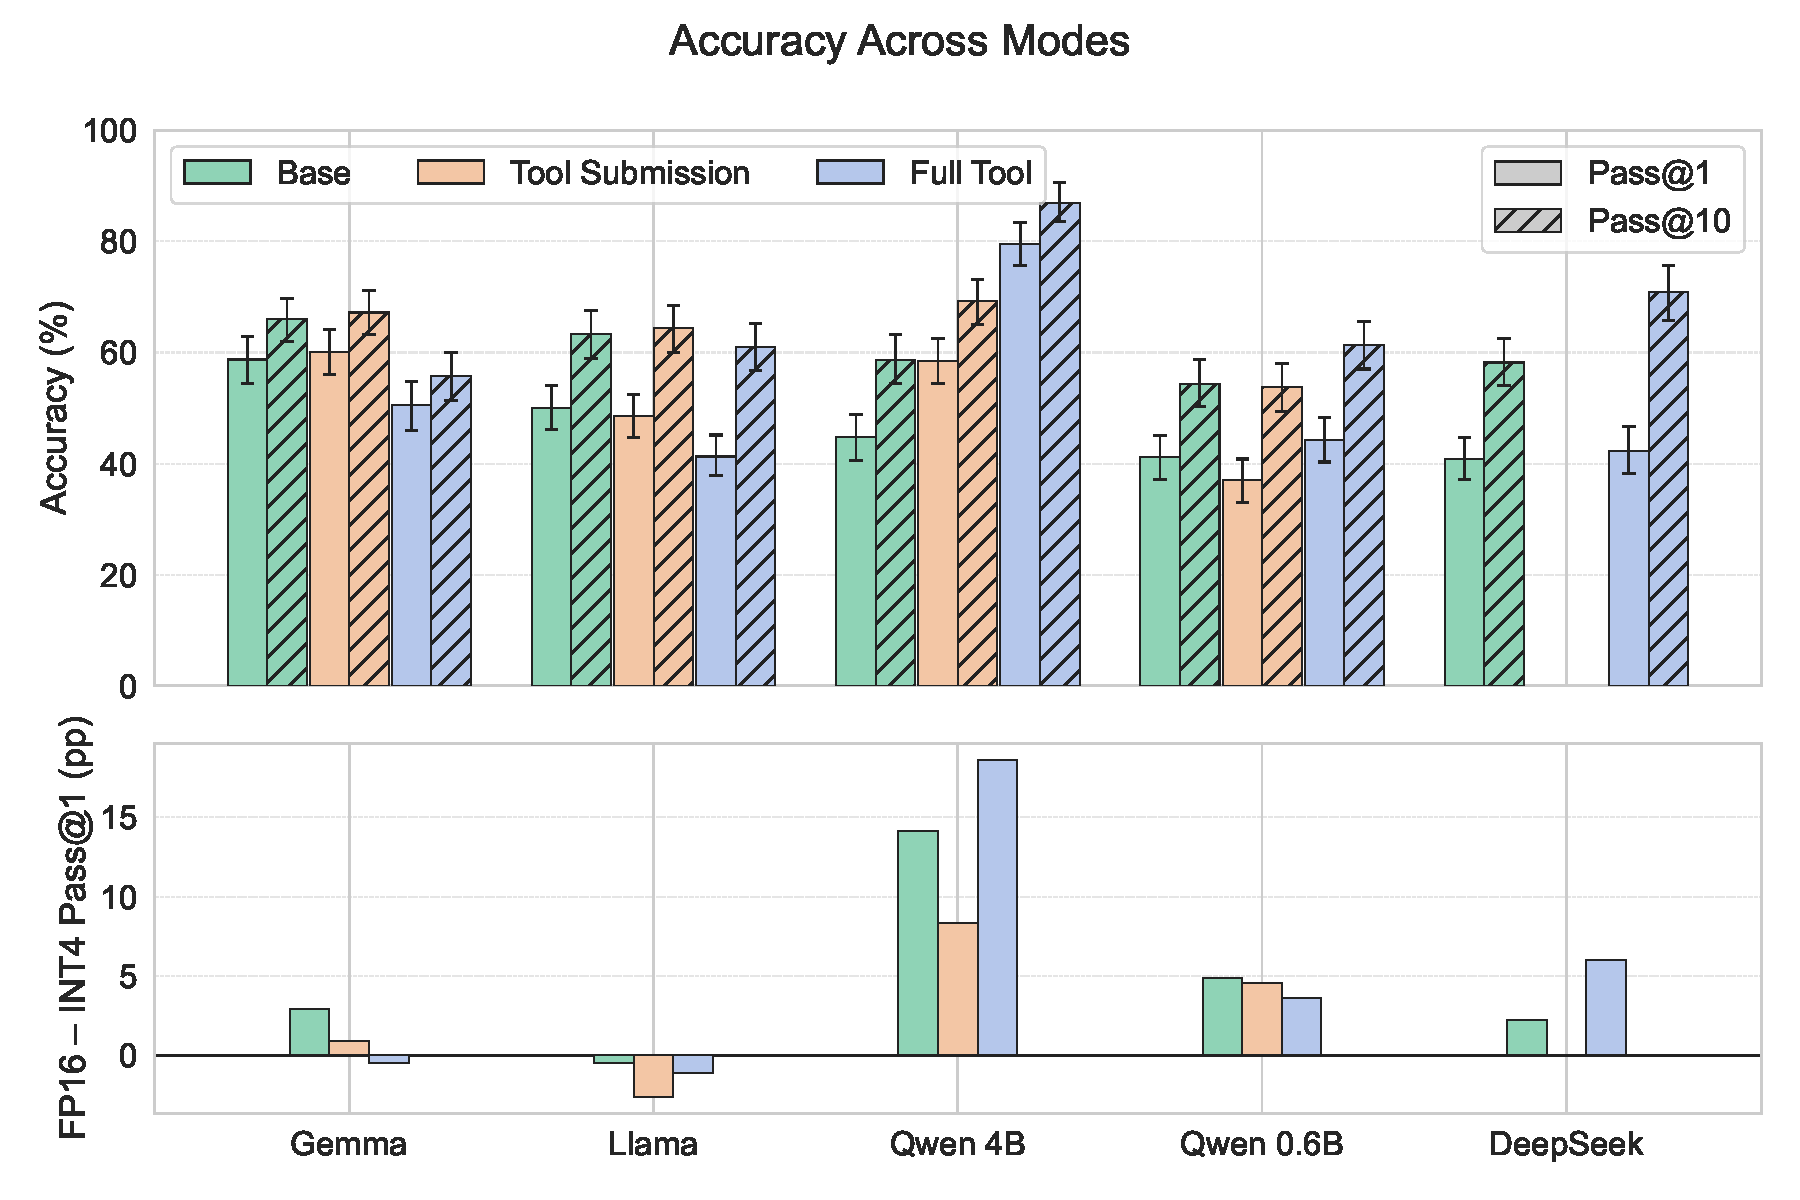
\includegraphics[width=\linewidth]{figs/final/accuracy_fp16.pdf}
    \caption{Pass@1 Accuracy}
    \label{fig:accuracy}
  \end{subfigure}
  \hfill
  \begin{subfigure}[b]{0.46\textwidth}
    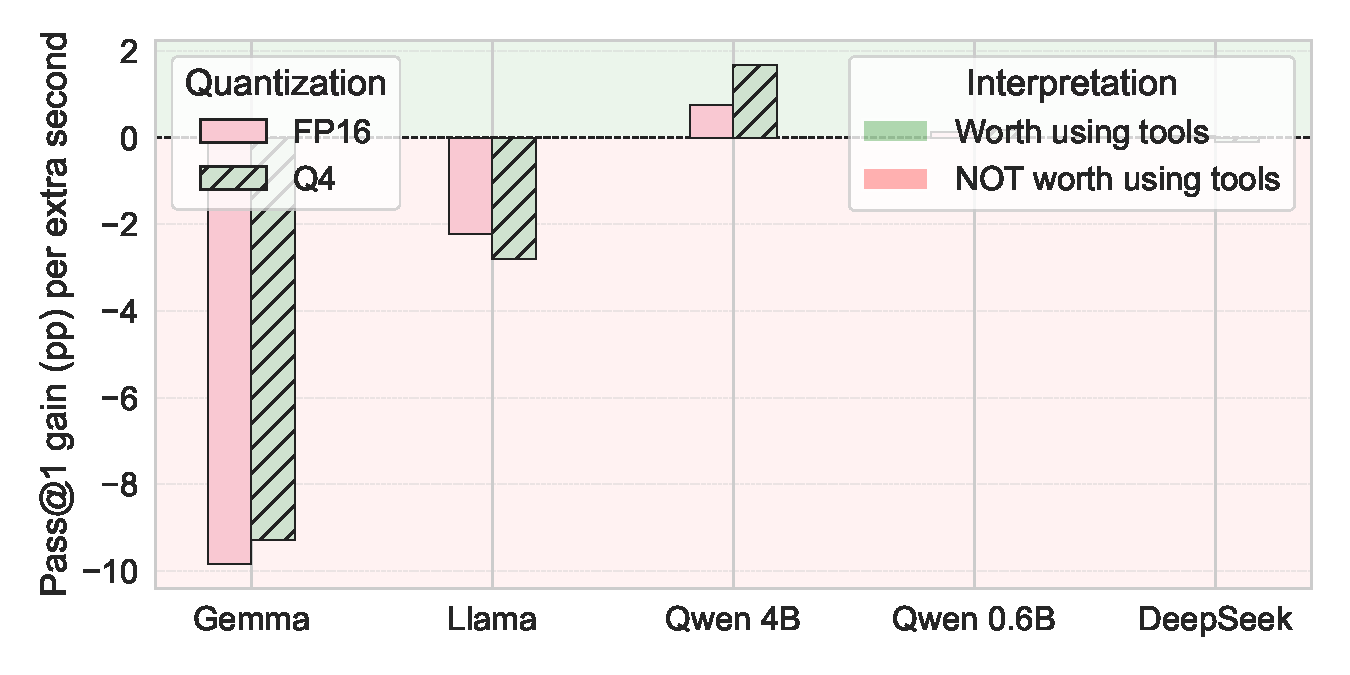
\includegraphics[width=\linewidth]{figs/final/tool_benefit.pdf}
    \caption{Tool Benefit Index}
    \label{fig:tool-benefit}
  \end{subfigure}
  \caption{Agent Effectiveness Analysis. (a) Pass@1 accuracy across models and execution modes. Qwen 3 (4B) benefits strongly from agency. (b) Tool benefit index (Pass@1 gain per second of latency). Only Qwen models deliver positive returns.}
  \label{fig:effectiveness}
  \Description{Panel (a) presents Pass@1 accuracy for several language models evaluated in Base, Tool-Submission, and Full-Tool modes. The top part reports FP16 results, showing that only Qwen 3 4B achieves a substantial gain from Full-Tool execution. The lower part plots FP16 minus INT4 accuracy differences. Panel (b) shows the tool benefit index on an A100 GPU, computed as Pass@1 improvement per additional second of latency. Gemma 3n and Llama 3.2 exhibit negative returns, while Qwen 3 4B achieves positive benefit.}
\end{figure*}

Figure~\ref{fig:accuracy} shows Pass@N accuracy across models and modes. Qwen 3 (4B) exhibits a clear capability threshold,, i.e., Pass@1 jumps from 44.8\% (95\% CI $[40.6,48.9]$) in Base mode to 79.6\% ($[75.7,83.4]$) in Full-Tool mode, and Pass@10 reaches 86.9\%. Qwen 3 (0.6B) posts only a modest gain (41.2\% $\rightarrow$ 44.3\%), while Gemma 3n and Llama 3.2 lose accuracy when tools are enabled (58.7\% $\rightarrow$ 50.5\% and 50.1\% $\rightarrow$ 41.3\%, respectively). DeepSeek R1 shows very slight performance improvements from 40.7\% to 42.2\% but requires substantially longer runtimes (described further in Section~\ref{sec:energy-thermals}). Aggregating over the repeated-attempt protocol (described in Section~\ref{sec:setup}), Qwen 3 (4B) also raises its per-attempt success probability from 11.0\% (CI $[9.9,12.3]$) to 35.1\% (CI $[32.1,38.3]$), whereas the other models see at most minor shifts. Interestingly, even after comprehensive iteration of the runtime and the prompt, DeepSeek R1 is unable to produce valid tool calls in the Tool-Submission mode, resulting in a Pass@1 rate of 0\% (the model frequently produces malformed JSON with missing or incorrectly nested fields, or tries to output Python code directly as a response). The bottom subfigure of Figure~\ref{fig:accuracy} illustrates the difference in Pass@1 performance between the INT4 quantized and FP16 versions of each model. Interestingly, Qwen 3 (4B) stands out strongly as the model most affected by radical integer quantization.

To analyze the tool benefit index, which requires robust 10-sample Pass@k statistics, we use results from the A100 platform. Figure~\ref{fig:tool-benefit} presents the tool benefit index, defined by the quotient of Pass@1 gain between the base and Full-Tool modes and the caused extra latency. Even on the server, the return on agency is limited: Qwen 3 (4B) gains 34.8 percentage points of Pass@1 for 46.5 extra seconds (0.75 pp/s), while Qwen 3 (0.6B) trades 3.1 percentage points for 22.8 seconds (0.14 pp/s). Llama 3.2 and Gemma 3n lose 8-9 percentage points despite longer attempts, while DeepSeek R1 shows only a fractional improvement despite an additional 30 seconds per try on average.

These trends suggest that tool-augmented agency is only beneficial for models that already produce coherent plans and tool calls. Comparing Gemma-3n against Qwen 3 (4B), it is evident that tool augmentation and added agency help reasoning models more.  In practice, we find that agents should begin in Base or Tool-Submission modes and progress to Full-Tool operation only when the observed tasks and confidence warrant the additional 20-50 s latency penalty. We also observe repeated tool invocations and malformed actions from the weaker models, underscoring the need for tool call caches, and training signals that prioritize syntactic correctness over raw tool-call volume.

\begin{insightbox}{Capability is a prerequisite for agency}
Agency is not a universal enhancement; it is an emergent property of model capability. Deploying agentic frameworks with under-provisioned models harms performance without any of the benefits.
\end{insightbox}

\subsection{Anatomy of Agentic Overhead}

\begin{figure*}[t]
\centering
\begin{subfigure}[b]{0.48\textwidth}
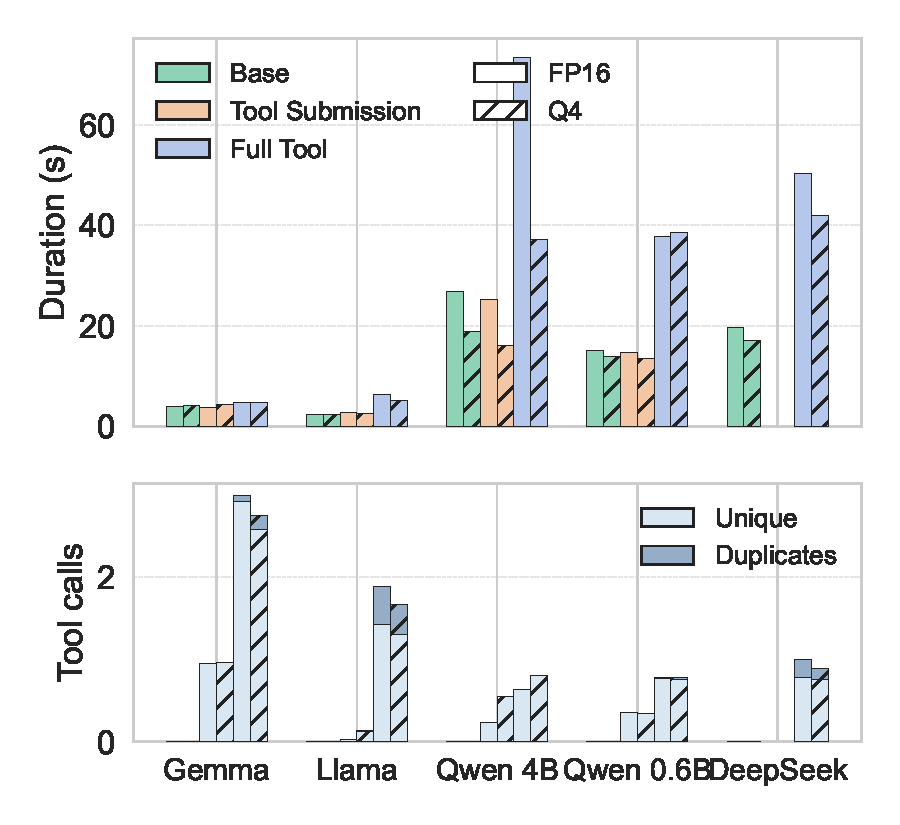
\includegraphics[width=\linewidth]{figs/final/overhead_breakdown.pdf}
\caption{Latency and Tool Calls}
\label{fig:overhead-breakdown}
\end{subfigure}
\hfill
\begin{subfigure}[b]{0.48\textwidth}
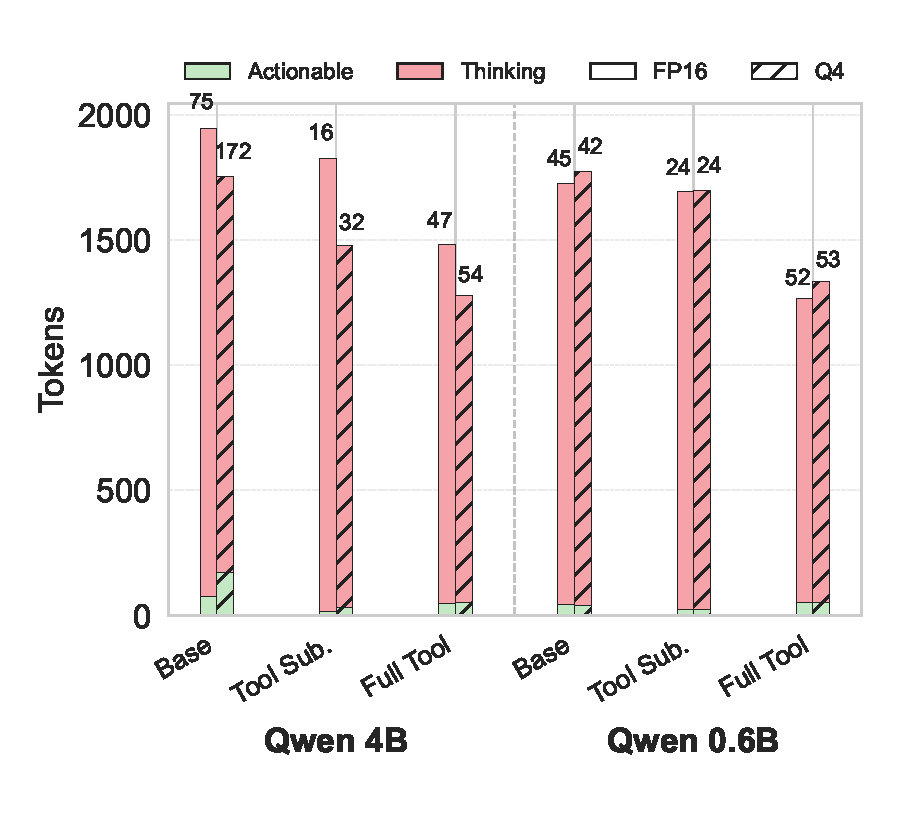
\includegraphics[width=\linewidth]{figs/final/thinking_share_qwen3_4b.pdf}
\caption{Thinking Token Share}
\label{fig:thinking-pie}
\end{subfigure}
\caption{Agentic Overhead Analysis. (a) End-to-end time and tool-call volume on A100. Full-Tool mode increases duration by 2-3$\times$. (b) Token distribution in thinking models. Thinking tokens dominate output, often exceeding 90\%.}
\label{fig:overhead}
\Description{Panel (a) summarizes runtime and tool-call behaviors. The top chart reports mean attempt duration, showing Full-Tool execution substantially increases runtime. The bottom chart presents the number of tool calls issued per attempt. Panel (b) shows the distribution of actionable tokens versus thinking tokens for Qwen models. Thinking tokens dominate model outputs, often exceeding 90\% of the total generation, while actionable tokens remain a small fraction.}
\end{figure*}

Figure~\ref{fig:overhead-breakdown} shows that, on the A100 evaluation, Full-Tool mode stretches mean attempt duration by roughly 2-3$\times$ for every model. Qwen 3 (4B) average submission increases from 26.9s to 73.4s in FP16 (18.9s to 37.1s in Q4\_K\_M), Qwen 3 (0.6B) from 15.0s to 37.8s, and DeepSeek R1 from 19.6s to 50.4s. Gemma 3n is comparatively insensitive (3.9s $\rightarrow$ 4.8s), which is surprising as it shows the largest number of total tool calls. This is caused by Gemma often issuing tool calls that require only a short list of parameters, such as listing available files, and generally making the submission from its generated file, rather than typing it out again. Llama 3.2 issues 1.9 calls but repeats roughly a quarter of them, whereas the Qwen models stay below one call. The bottom subfigure includes tool calls from the failed attempts. This fact, combined with Qwen models' relatively high pass-rates, suggests that most of the failures are actually caused by failed tool calls, rather than incorrect submissions.


Table~\ref{tab:platform-tps} shows a $18.7\times$ performance variation across platforms. The iPhone 16 Pro achieves $2.6 \times$ the OnePlus 10 Pro's throughput, highlighting the efficiency of Apple's tightly integrated SoC. Furthermore, the newer iPhone 16 Pro achieves $1.5\times$ better throughput compared to iPhone 15, demonstrating the newer, more powerful SoC and larger memory. The A100 provides data-center-class inference speed at $2.3 \times$ the speed of the high-end laptop MacBook Pro, suggesting that for inference-speed critical applications, cloud inference remains unmatched.


To understand the trade-offs between latency and energy efficiency, we extended our experiments with a prefill testing mode that sweeps 50-3500-token prompts (increments of 50-tokens) drawn from a pool of single-token words, while disabling \texttt{llama.cpp} prefix caching.
We discard five warm-up prompts and then record twenty repetitions per length, logging TTFT and memory pressure on the MacBook M2 Max.
Figure~\ref{fig:prefill-qwen} illustrates the resulting prefill latency curves, showing a near-linear relationship between the TTFT and the prompt length, with the mobile tests showing a significant higher gradient in the relationship. The longest prompts tested without memory overflow issues on the iPhone 15 were 1800 tokens, which demonstrated a near-five-minute prefill stage, which is completely prohibitive for most applications. The vertical lines drawn in the figure at 460 and 1550 tokens are the lengths of the prompts used in the Base and Full-Tool modes, respectively. These curves show that for both platforms, the TTFT increases by more than 100\%; on Qwen 3 (0.6B) from 182ms to 358ms, and on Qwen 3 (4B) from 737ms to 2.11s. On mobile, this effect is exemplified, as the TTFT of Qwen 3 (4B) is increased by $\approx 3.5\times$, resulting in a more than 4.5-minute TTFT for the Full-Tool mode. Without effective context management, the prefill stage quickly dominates end-to-end latency, motivating the use of warm KV and prefix caches, as well as tool and prompt trimming.

\begin{insightbox}{Prefill Dominates Post-Tool Latency}
For on-device agents, the dominant performance bottleneck is not the tool's execution time but the cost of prefilling the initial longer prompts. Limited memory and parallelism on mobile devices exacerbate this effect, making context management a more critical optimization than tool performance itself.
\end{insightbox}

\subsection{Quantization Paradox (Architecture-dependent)}
\label{sec:quantization}



\begin{table*}[ht]
\centering
\begin{minipage}{0.35\textwidth}
\centering
\caption{Cross-platform TPS comparison (Qwen 3 4B, INT4, Base mode).}
\label{tab:platform-tps}
\resizebox{\textwidth}{!}{%
\begin{tabular}{l r r}
\hline
\textbf{Platform} & \textbf{TPS} & \textbf{Relative} \\
\hline
OnePlus 10 Pro & 4.9 & $1.0\times$ \\
iPhone 15 & 8.6 & $1.8\times$ \\
iPhone 16 Pro & 12.5 & $2.6\times$ \\
MacBook M2 Max & 39.7 & $8.1\times$ \\
HPC A100 & 91.6 & $18.7\times$ \\
\hline
\end{tabular}%
}
\end{minipage}%
\hfill
\begin{minipage}{0.63\textwidth}
\centering
\caption{Precision comparison across platforms}
\label{tab:quantization}
\resizebox{\textwidth}{!}{%
\begin{tabular}{@{} l l l r r r @{}}
\hline
\textbf{Platform} & \textbf{Model} & \textbf{Precision} & \textbf{TPS} & \textbf{Power (W)} & \textbf{J/token} \\
\hline
MacBook M2 Max & Gemma 3n        & FP16      & 24.4 & 10.6 & 0.44 \\
MacBook M2 Max & Gemma 3n        & Q4\_K\_M  & 0.6  & 18.5 & 30.7 \\
MacBook M2 Max & Qwen 3 (4B)     & FP16      & 22.7 & 18.0 & 0.79 \\
MacBook M2 Max & Qwen 3 (4B)     & Q4\_K\_M  & 39.7 & 21.2 & 0.53 \\
\hline
HPC A100     & Gemma 3n        & FP16      & 58.4 & 4.5  & 0.11 \\
HPC A100     & Gemma 3n        & Q4\_K\_M  & 54.2 & 5.0  & 0.13 \\
HPC A100     & Qwen 3 (4B)     & FP16      & 71.3 & 10.1 & 0.14 \\
HPC A100     & Qwen 3 (4B)     & Q4\_K\_M  & 91.6 & 9.7  & 0.11 \\
HPC A100     & DeepSeek R1     & FP16      & 96.8 & 9.7  & 0.10 \\
HPC A100     & DeepSeek R1     & Q4\_K\_M  & 115.0& 9.6  & 0.08 \\
\hline
\end{tabular}%
}
\end{minipage}
\vspace{-0.4em}
\begin{flushleft}\scriptsize
Gemma 3n INT4 on the Mac executes via a CPU fallback path, hence the annotated energy spike.
\end{flushleft}
\end{table*}

Table~\ref{tab:quantization} and Figure~\ref{fig:quant-inversion} show the combined MacBook M2 Max and A100 measurements. On the Mac, Qwen 3 (4B) benefits from INT4 (22.7 $\rightarrow$ 39.7 TPS, with energy per token dropping from 0.79~J to 0.53~J), but Gemma's Q4 checkpoint collapses to 0.6~TPS and 30.7~J/token. Inspection of the \texttt{llama.cpp} logs and powermetrics traces confirmed that Gemma INT4 currently falls back to a CPU matmul path because no Metal kernel is supplied by the runtime, leaving the GPU mostly idle while the CPU package draws $\approx$ 18~W. This implementation gap may stem from model-specific layer configurations. In this case, we suspect that the reason for Gemma's performance degradation is its sliding window attention patterns, which are not yet supported by the \texttt{llama.cpp}'s generic INT4 quantization kernels for Metal. The Mac energy subplot is therefore clipped and annotated.

On the NVIDIA A100, where \texttt{llama.cpp} provides native INT4 CUDA kernels, the results are that Q4\_K\_M delivers 1.3$\times$ higher throughput and roughly 20-30\% lower energy per token across all models. The cross-platform contrast highlights the need to co-design quantization schemes with kernel availability and memory bandwidth.

\begin{insightbox}{Hardware-Aware Precision}
Match quantization to kernel support. INT4 accelerates models that ship native GPU kernels (Qwen, DeepSeek), but falls back to slower CPU execution when those kernels are absent (Gemma), erasing any efficiency gains.
\end{insightbox}


\subsection{Energy \& Thermals}
\label{sec:energy-thermals}

\begin{figure*}[t]
  \centering
  \begin{subfigure}[b]{0.32\textwidth}
    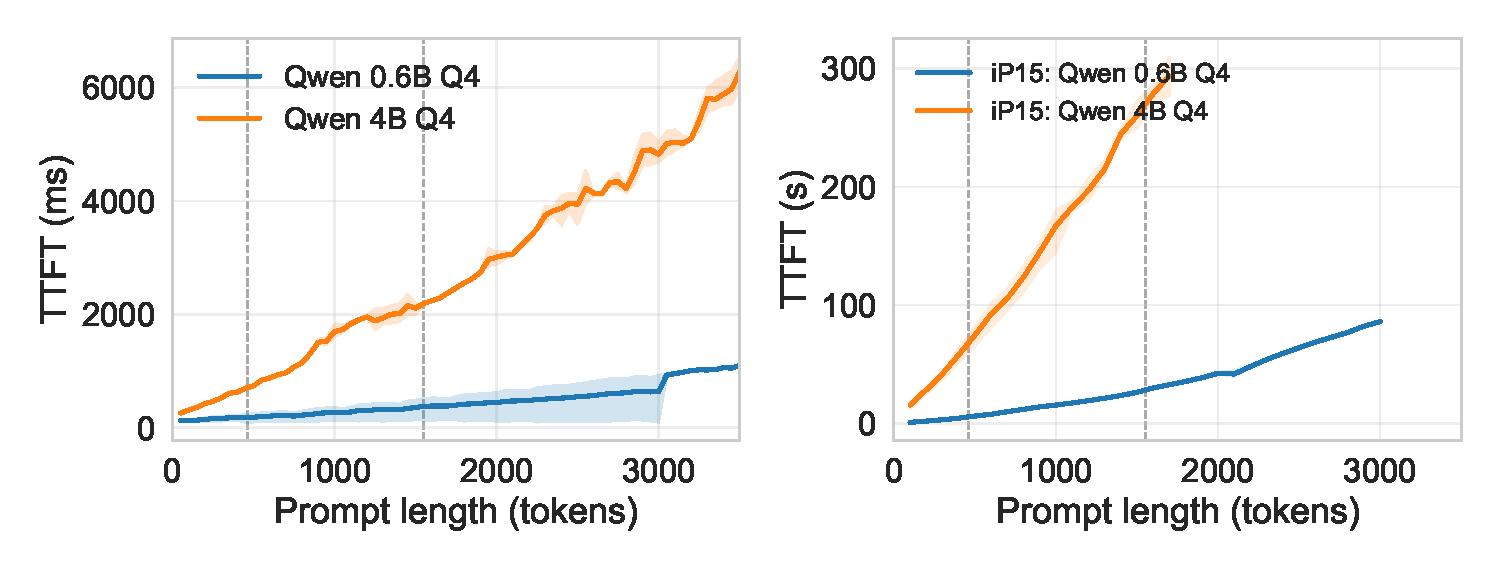
\includegraphics[width=\linewidth]{figs/final/prefill_qwen.pdf}
    \caption{Prefill Latency (TTFT)}
    \label{fig:prefill-qwen}
  \end{subfigure}
  \hfill
  \begin{subfigure}[b]{0.32\textwidth}
    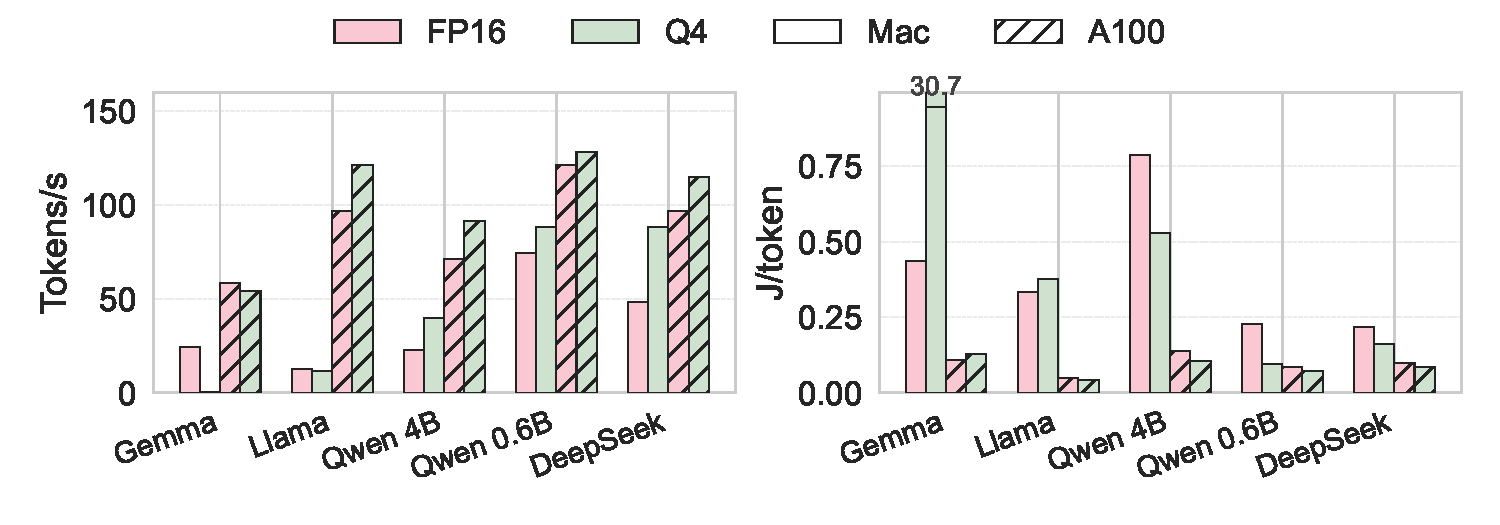
\includegraphics[width=\linewidth]{figs/final/quantization_a100.pdf}
    \caption{Throughput \& Energy/Token}
    \label{fig:quant-inversion}
  \end{subfigure}
  \hfill
  \begin{subfigure}[b]{0.32\textwidth}
    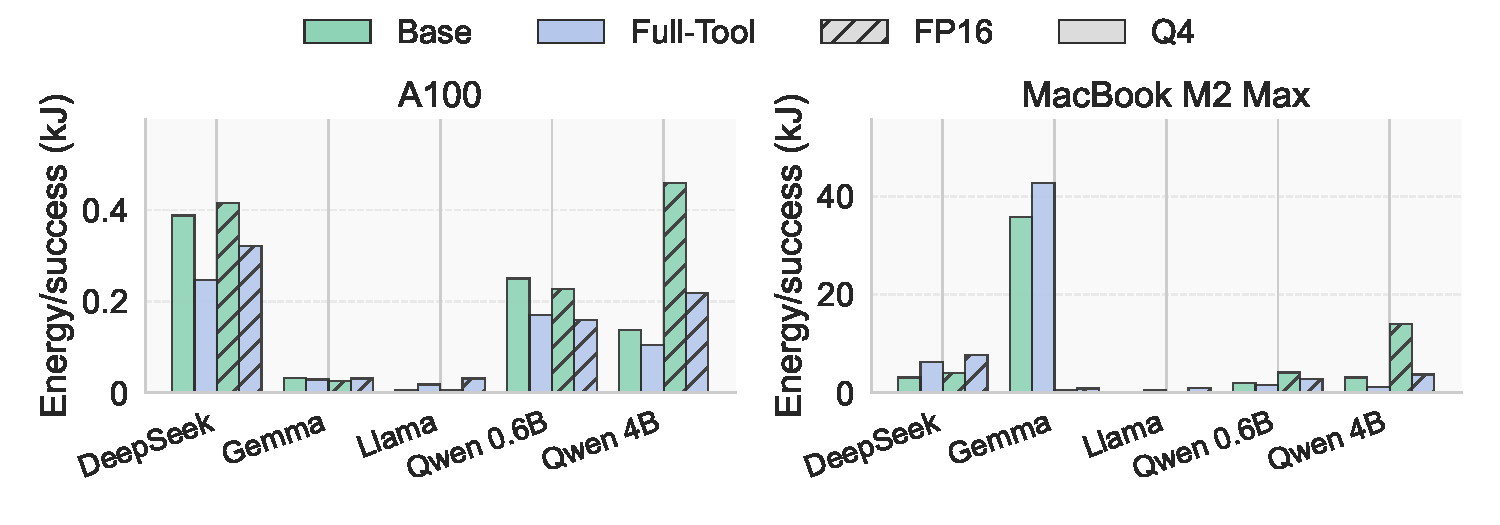
\includegraphics[width=\linewidth]{figs/final/energy_per_success_panels.pdf}
    \caption{Energy per Success}
    \label{fig:energy-per-success}
  \end{subfigure}
  \caption{Performance and Energy Analysis. (a) Prefill latency dominates on mobile for long prompts. (b) Quantization benefits depend on kernel support (Gemma INT4 regression). (c) Energy-per-success reveals the "inverse efficiency paradox" where mobile is least efficient.}
  \label{fig:combined-perf-energy}
  \Description{Panel (a) shows prefill latency vs prompt length, highlighting mobile bottlenecks. Panel (b) compares throughput and energy per token across platforms and precisions. Panel (c) shows the total energy required to solve a task, with mobile devices consuming the most energy.}
\end{figure*}

Figure~\ref{fig:energy-per-success} presents the energy-per-success metric across three platforms. On A100, Qwen 3 (4B) drops from 0.46 to 0.22kJ with tools as mean attempts fall (2.01$\rightarrow$1.35) and per-attempt energy declines (270$\rightarrow$205J). Qwen 3 (0.6B) yields a smaller gain (0.25$\rightarrow$0.17kJ), whereas Gemma 3n and Llama-3.2 use comparable or more energy with tools, because Pass@1 decreases and required attempts rise. DeepSeek R1 sits between the extremes: energy falls in both precisions (0.42$\rightarrow$0.32kJ FP16; 0.39$\rightarrow$0.25kJ Q4) but remains high due to long chains of thought.
On the MacBook, kernel availability dominates: Qwen 3 (4B) still improves the energy metric when using tools (14.07$\rightarrow$3.72kJ FP16; 3.09$\rightarrow$1.18kJ Q4), while DeepSeek R1 and Llama-3.2 again see a negative benefit in using tools (4.05$\rightarrow$7.65~kJ Q4; 0.14$\rightarrow$1.00~kJ FP16). Gemma 3n in Q4 increases to 36-43~kJ per solution due to the missing integer kernel (Section \ref{sec:quantization}).
On the iPhone 15, we observe similar trends with a larger difference between reasoning and non-reasoning models, as limited memory and parallelism make long responses costly. Overall, the three subfigures show that agentic efficiency is hardware-dependent: capable models benefit from tool-use on all tested platforms, but runtime differences can invert the benefit for otherwise solid architectures. Notably, we see an interesting observation: the energy-per-success is highest on mobile, lower on the MacBook, and lowest on the server. While the absolute mobile energy values are estimates (subject to the $\pm$15\% uncertainty described in Section~\ref{sec:setup}), the relative ranking between models and the massive gap compared to desktop/server platforms are robust signals that persist across repeated trials.

\begin{table}[!t]
\centering
\caption{Platform power characteristics}
\label{tab:power}
\setlength{\tabcolsep}{8pt}%
\renewcommand{\arraystretch}{1.15}%
\begin{tabular}{l r r r}
\hline
\textbf{Platform} & \textbf{Base (W)} & \textbf{Full-Tool (W)} & \textbf{Memory (GB)} \\
\hline
iPhone 15 & 7.2 & 8.3 & 6 \\
iPhone 16 Pro & 6.9 & 7.8 & 8 \\
OnePlus 10 Pro & 12.8 & 14.2 & 12 \\
MacBook M2 Max & 28.7 & 31.2 & 64 \\
HPC A100 & 110.8 & 115.3 & 40 (HBM2) \\
\hline
\end{tabular}
\end{table}

On the MacBook Pro (M2 Max), the \emph{generation-phase} power averages 28.7W (base) to 31.2W (Full-Tool) as shown in Table~\ref{tab:power}. On the A100, active generation power averages roughly 110W; the extra wall-clock time in Full-Tool mode therefore includes periods of reduced power draw during tool execution and result processing.
Our thermal- and battery-aware scheduling (described in Section~\ref{sec:setup}) prevents throttling. Without this mitigation, the OnePlus 10 Pro experiences 31\% performance degradation after 90 seconds, while iPhones maintain stable performance for 180 seconds due to superior thermal design.

\begin{insightbox}{Optimize for Task Success, Not Just Inference Speed}
For capable on-device agents, the total energy-to-solution is dominated by the number of attempts required for success, and the average length of the responses. This supports employing more computationally expensive models or reasoning steps, if they significantly increase the first-pass success rate.
\end{insightbox}

\subsection{The Cost of Thought (CoT)}
\label{sec:cost_of_thought}

Figure~\ref{fig:thinking-pie} shows that the Qwen thinking models devote nearly all of their output to internal deliberation on MBPP. In FP16 Base mode, Qwen 3 (4B) emits $\approx$1,871 thinking tokens versus only 75 actionable tokens (96\% thinking share), and Full-Tool mode still spends $\approx$1,437 tokens reasoning before producing 47 actionable tokens. Qwen 3 (0.6B) behaves similarly ($\approx$1,681 thinking vs. 45 actionable tokens in Base mode). In contrast, Gemma 3n produces about 160 actionable tokens with no dedicated reasoning stream, illustrating the $\approx 12 \times$ verbosity delta between chain-of-thought and non-chain-of-thought models.

Longer traces, however, correlate with \emph{worse} outcomes. Across MBPP we measure negative Pearson correlations between thinking-token count and success for every Qwen configuration: -0.68/-0.67/-0.56 for Qwen 3 (4B) FP16 in base/tool-sub/full-tool, and -0.69/-0.76/-0.49 for the corresponding Q4\_K\_M runs. Qwen 3 (0.6B) shows the same trend with slightly weaker slopes (-0.44/-0.40/-0.20 in FP16; -0.45/-0.35/-0.17 in Q4\_K\_M). Successful attempts therefore wrap up after roughly one thousand thinking tokens, whereas failures meander for 1.3–2.0k tokens. The chains are long because the model is stuck, not because it is refining a better answer, motivating summarization, or gating mechanisms that terminate unproductive reasoning loops sooner.

\begin{insightbox}{Verbosity Drives Energy Cost}
On resource-constrained devices, long chain-of-thought traces primarily consume energy and time rather than improving outcomes. Keeping prompts compact is therefore a first-order systems concern.
\end{insightbox}

\subsection{Networking Overhead}
\label{sec:networking}

For hybrid or cloud-offloaded agents, network latency is often cited as a bottleneck. However, our results suggest that for complex agentic workloads, the network Round-Trip Time (RTT) is effectively negligible.
Literature suggests typical RTTs of 20-50ms for WiFi, 30-70ms for 5G, and 50-100ms for 4G LTE \cite{huang20225g_latency, parvez2018survey_latency}. Even with application-layer overheads doubling these values to $\approx$300ms, this latency constitutes less than 1\% of the 30–70s end-to-end duration of a typical agentic loop (Figure~\ref{fig:overhead}a).
[TODO: Insert actual measured RTT and payload transfer times for our specific tool payloads].
Thus, for computationally intensive agentic tasks, the decision to offload should be driven by privacy, cost, and availability constraints rather than latency concerns.

Beyond latency, the energy cost of radio usage is significant. Cellular radios incur high "tail energy" costs, remaining in high-power states for seconds after transmission finishes \cite{huang2012close_look_power}. For an agentic loop with frequent, small tool exchanges, this can lead to the radio remaining in a high-power state continuously, negating the benefits of idle periods.
[TODO: Insert estimated radio energy cost based on packet size and tail state models].

\section{Discussion}
Our measurement insights highlight cross-layer considerations for deployable LLM agency on resource-constrained devices.

\textbf{Systems.} Prefill and cache maintenance dominate the loop cost once prompts grow beyond 1.5k tokens (as shown in Figures~\ref{fig:overhead-breakdown} and~\ref{fig:prefill-qwen}). Tool-aware runtimes should therefore maintain KV caches, trim stale turns, and couple quantization choices with kernel availability to avoid the regressions we observe on Gemma INT4. These observations suggest that runtime co-design should focus not only on raw throughput, but also on effective context management, memory bandwidth provisioning, and hardware-aware quantization. Extending Pocket Agent to additional SoCs such as Google Tensor and Samsung Exynos will provide deeper insights into platform-specific trade-offs, helping us understand whether our insights hold across an even broader set of consumer devices.

\textbf{Applications.} Uneven tool benefits (shown in Figure~\ref{fig:tool-benefit}) suggest that indiscriminate "agentification" is harmful. Rather than simply exposing tools, applications must implement \textit{capability-gated agency}: starting in a low-latency Base mode and escalating to Full-Tool operation only when the model's self-assessed confidence is low or the task complexity warrants the 20–50~s latency penalty.
While our study focuses on fully on-device execution, real-world deployments are likely to involve hybrid settings where local inference is complemented by selective cloud offloading. Incorporating such hybrid configurations into Pocket Agent would allow a more complete accounting of end-to-end deployment feasibility, including both computation and communication costs.
The "Network Tax" is therefore primarily energetic and privacy-related, not temporal. While cloud inference is significantly faster (18.7$\times$ throughput), the energy cost of radio usage and the privacy risks of data transmission remain the primary motivators for local execution. For latency-critical but simple tasks, the network overhead matters; for complex agentic reasoning, the cloud's speed advantage overwhelmingly amortizes the RTT.


\textbf{Models.} Energy-to-solution improves when tool calls are correct and chains of thought remain concise (as shown in Figures~\ref{fig:energy-per-success} and \ref{fig:thinking-pie}). Training signals that reward syntactic accuracy and gate unproductive reasoning will convert Tool$\rightarrow$Action$\rightarrow$Observation loops into tangible gains on battery-powered devices.
Our analysis also shows that verbosity strongly correlates with wasted energy, which highlights the importance of model-level interventions such as reasoning summarization or adaptive chain-of-thought gating. As reasoning-centric models continue to evolve rapidly, repeating our evaluation on newer architectures will test the robustness of our conclusions and help refine model training strategies for agentic settings.

\textbf{Workload.} We choose the MBPP dataset for our evaluation because it provides reliable correctness verification and a controlled setting to measure tool overhead.
This allows us to precisely isolate the computational trade-offs of agentic loops.
Meanwhile, it opens an opportunity to extend Pocket Agent to broader domains, such as HumanEval, APPS, web navigation, instruction following, or retrieval-heavy agents involve different tools, interaction patterns, and verification protocols. Extending Pocket Agent to cover these workloads is therefore an exciting direction, and will help determine whether the observed capability thresholds, prefill bottlenecks, and energy-to-solution economics generalize beyond programmatic code generation.

Taken together, our findings highlight that on-device LLM agency is fundamentally a co-design challenge. Hardware and runtimes must move beyond peak token throughput to address prefill latency and memory bandwidth for long contexts. Applications must move beyond static tool definitions to dynamic, capability-gated invocation strategies. And models must evolve from maximizing reasoning length to optimizing the "energy-per-insight" ratio.


\section{Conclusion}
We contribute Pocket Agent, a comprehensive measurement framework designed to quantify the end-to-end cost of on-device LLM agency.
To address the challenges of deployment of LLM agents on resource-constrained devices, Pocket Agent enables measurement of the complete loop of Tool $\rightarrow$ Action $\rightarrow$ Observation.
We find that full tool-use increases runtime by 2–3$\times$ on mobile platforms, and that chain-of-thought reasoning, widely celebrated in the cloud, devotes up to 99\% of tokens to internal deliberation with little actionable output.
We further reveal an energy paradox, i.e., devices with the tightest resource budgets, such as smartphones, consume the most energy per solved task, while laptops and servers are progressively more efficient. These findings underscore that only sufficiently capable models benefit from tool use, that prefill and context growth dominate latency, and that energy-to-solution depends as much on accuracy as throughput. We also highlight the non-trivial role of networking, where latency and radio tail energy can significantly impact the viability of hybrid or cloud-tethered agents. Pocket Agent provides the first open-source framework to quantify these trade-offs, paving the way to develop efficient, privacy-preserving AI assistants on everyday devices.
As future research, we plan to extend our measurements to emerging small language models explicitly fine-tuned for agentic workloads. Evaluating such models with Pocket Agent will provide a more complete picture of how lightweight agents can be deployed efficiently at the edge in pervasive environments. Additionally, incorporating hybrid cloud-edge execution strategies and investigating dynamic tool selection mechanisms based on runtime resource availability represent promising directions.
Further exploration of diverse, multimodal agentic workloads together with cross-platform optimization techniques will help establish design principles for the next generation of pervasive AI systems.

\bibliographystyle{ACM-Reference-Format}
\bibliography{main}

\end{document}
